\graphicspath{{Figures/}}

\section{Results}

Using all the ingredients describe above we are able to compute the \ups \Raa as a function of the collision centrality and the rapidity.
The results are shown on the figure \ref{raaAlice} and compared to the previous ALICE results obtained at lower energy.
The ratio of ALICE results 5 TeV / 2.76 TeV is shown on the figure \ref{ratio}.
The large uncertainties leads to a ratio compatible with unity nevertheless we observe a systematic increase of the $\Raa$.
Finally, the results are compared to theoretical predictions (transport model) on the figure \ref{rapp} and \ref{kai}. 
The \Raa values are reported in the table \ref{raavaluescent} and \ref{raavaluesy}.

%The formula to calculate the nuclear modification factor is defined as,
%\begin{equation}
%  R_{\rm AA} = \frac{N_{\rm \Upsilon(1S)}}{(A\times\epsilon) \cdot \sigma_{pp} \cdot BR_{\varUpsilon(1S) \rightarrow \mu^{+}\mu^{-}} \cdot \langle T_{AA} \rangle \cdot N_{\rm MB}}
%\end{equation}
%
%\begin{equation*}
%  R_{\rm AA} = 0.39 \pm 0.03 \pm 0.04
%\end{equation*}
%using,
%\begin{eqnarray*}
%N_{\rm \Upsilon(1S)} & = & 1123 \pm 86 \pm 10 \\
%A\times\epsilon & = & (27.24 \pm 0.0 ) \% \\
%F_{norm} & = & 11.842 \pm 0.001 \pm 0.059 \\ 
%N_{CMUL7} & = & 127038461 \\
%T_{AA} & = & 6.22 \pm 0.2 \phantom{0} \mathrm{mb}^{-1} \\
%\sigma_{pp} \times BR_{\varUpsilon(1S) \rightarrow \mu^{+}\mu^{-}} & = & 1.14 \pm 0.10 \phantom{0} \mathrm{nb} \\
%\end{eqnarray*}
%\begin{center}
%  \scriptsize{Systematics : tracker : 3\%, trigger : 0.1\%, matching : 1\%, MC : 1\%, centrality : 2\%}
%\end{center}
%

\begin{figure}[!h]
  \centering 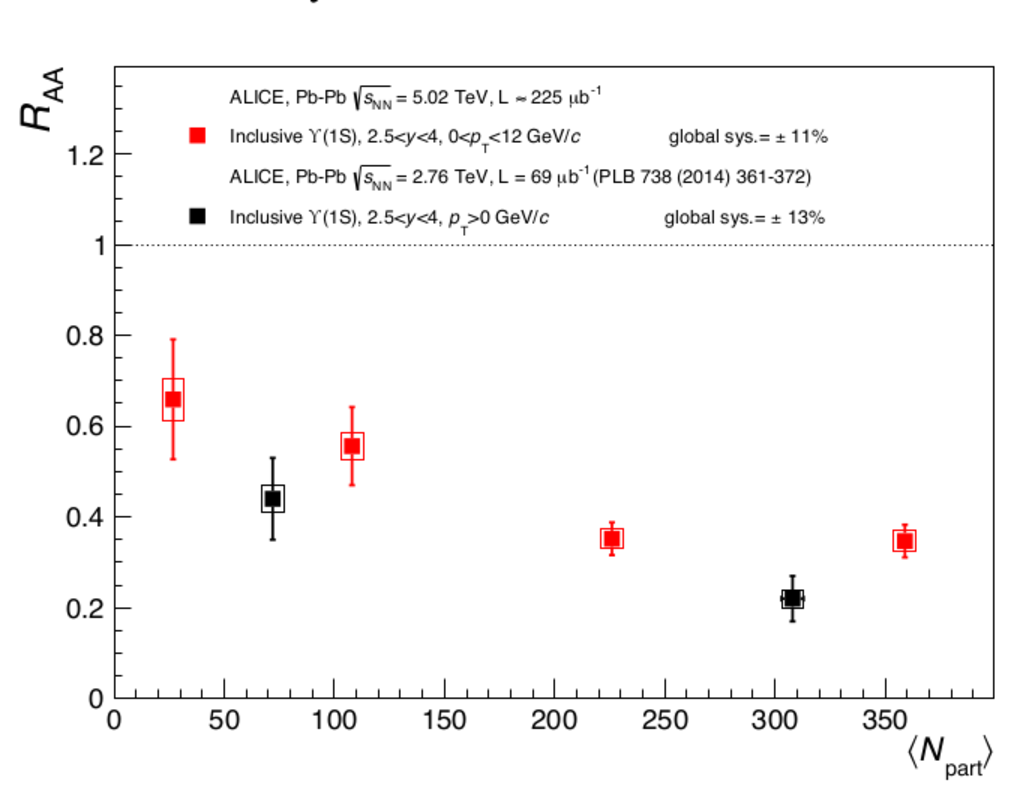
\includegraphics[width=6.5cm]{Results/Antoine_results_2016_06_07/RAA_vs_cent_5TeV_et_2760GeV.pdf}
  \centering 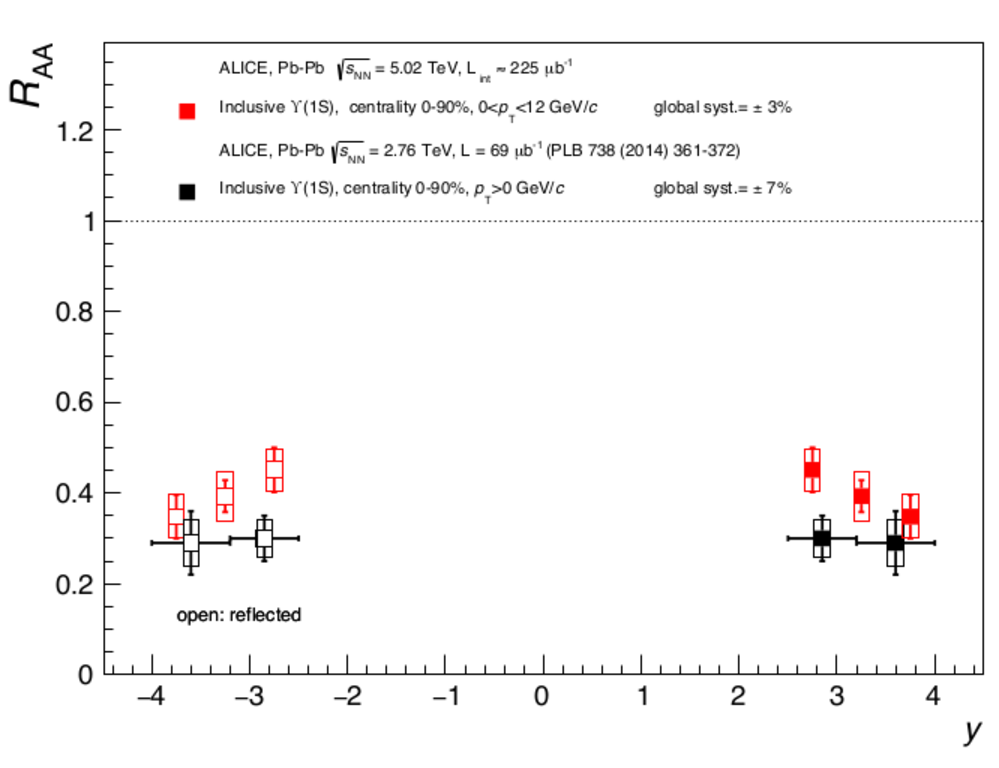
\includegraphics[width=6.5cm]{Results/Antoine_results_2016_06_07/RAA_vs_rap_5TeV_et_2760GeV.pdf}
  \caption{\label{raaAlice}\scriptsize $R_{\rm AA}$ vs centrality}
\end{figure}       

\begin{figure}[!h]
  \centering 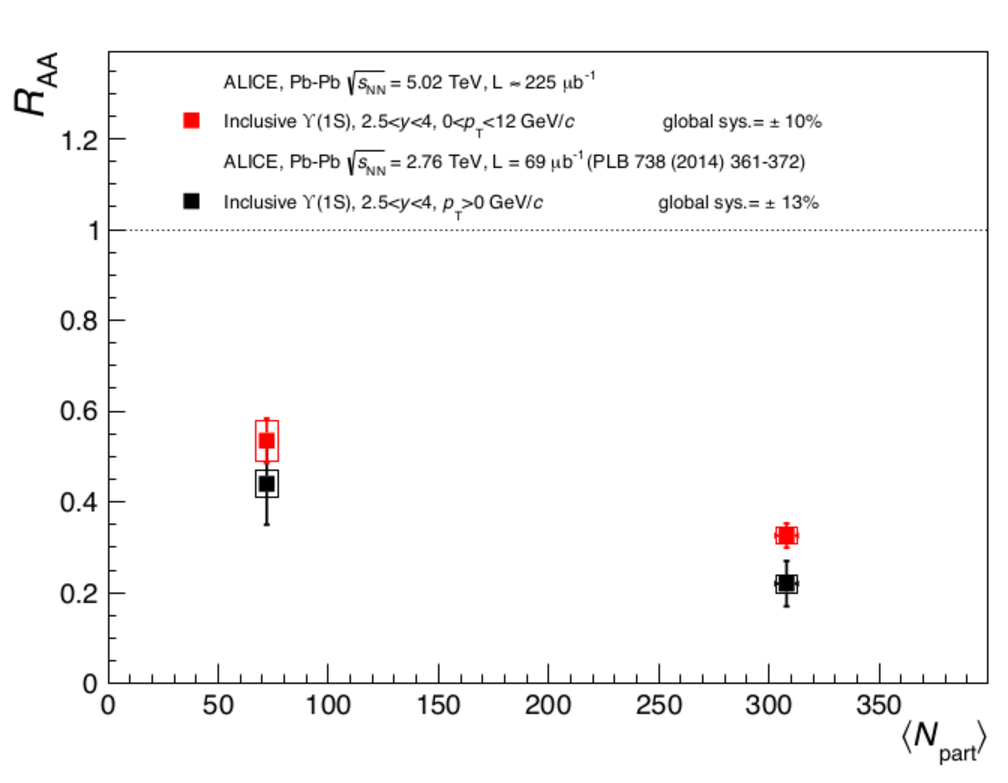
\includegraphics[width=6.5cm]{Results/Antoine_results_2016_06_07/RAA_vs_cent_5TeV_et_2760GeV_same_binning.pdf}
  \centering 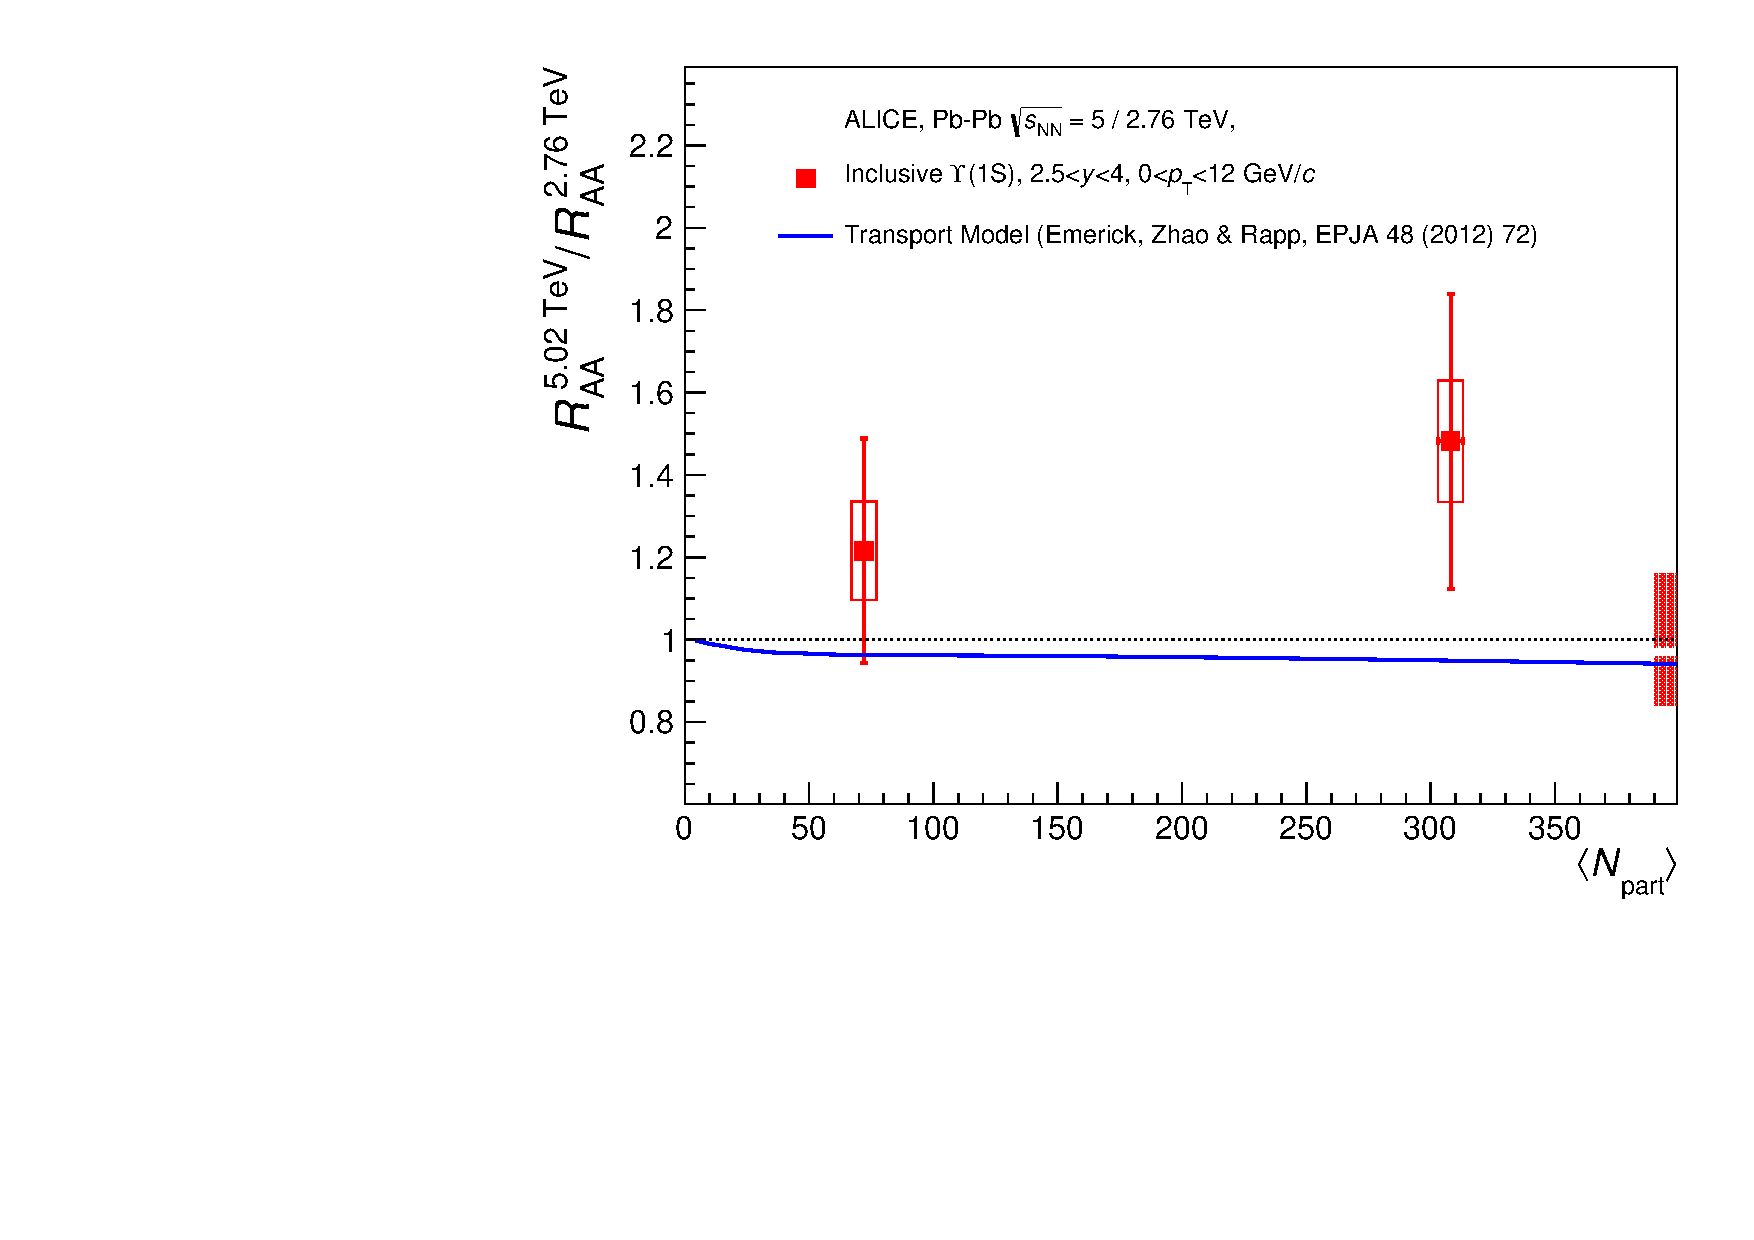
\includegraphics[width=6.5cm]{Results/Antoine_results_2016_06_07/RAA_vs_cent_5TeV_et_2760GeV_ratio.pdf}
  \caption{\label{ratio}\scriptsize $R_{\rm AA}$ vs centrality}
\end{figure}       

%\begin{figure}[!h]
%  \centering 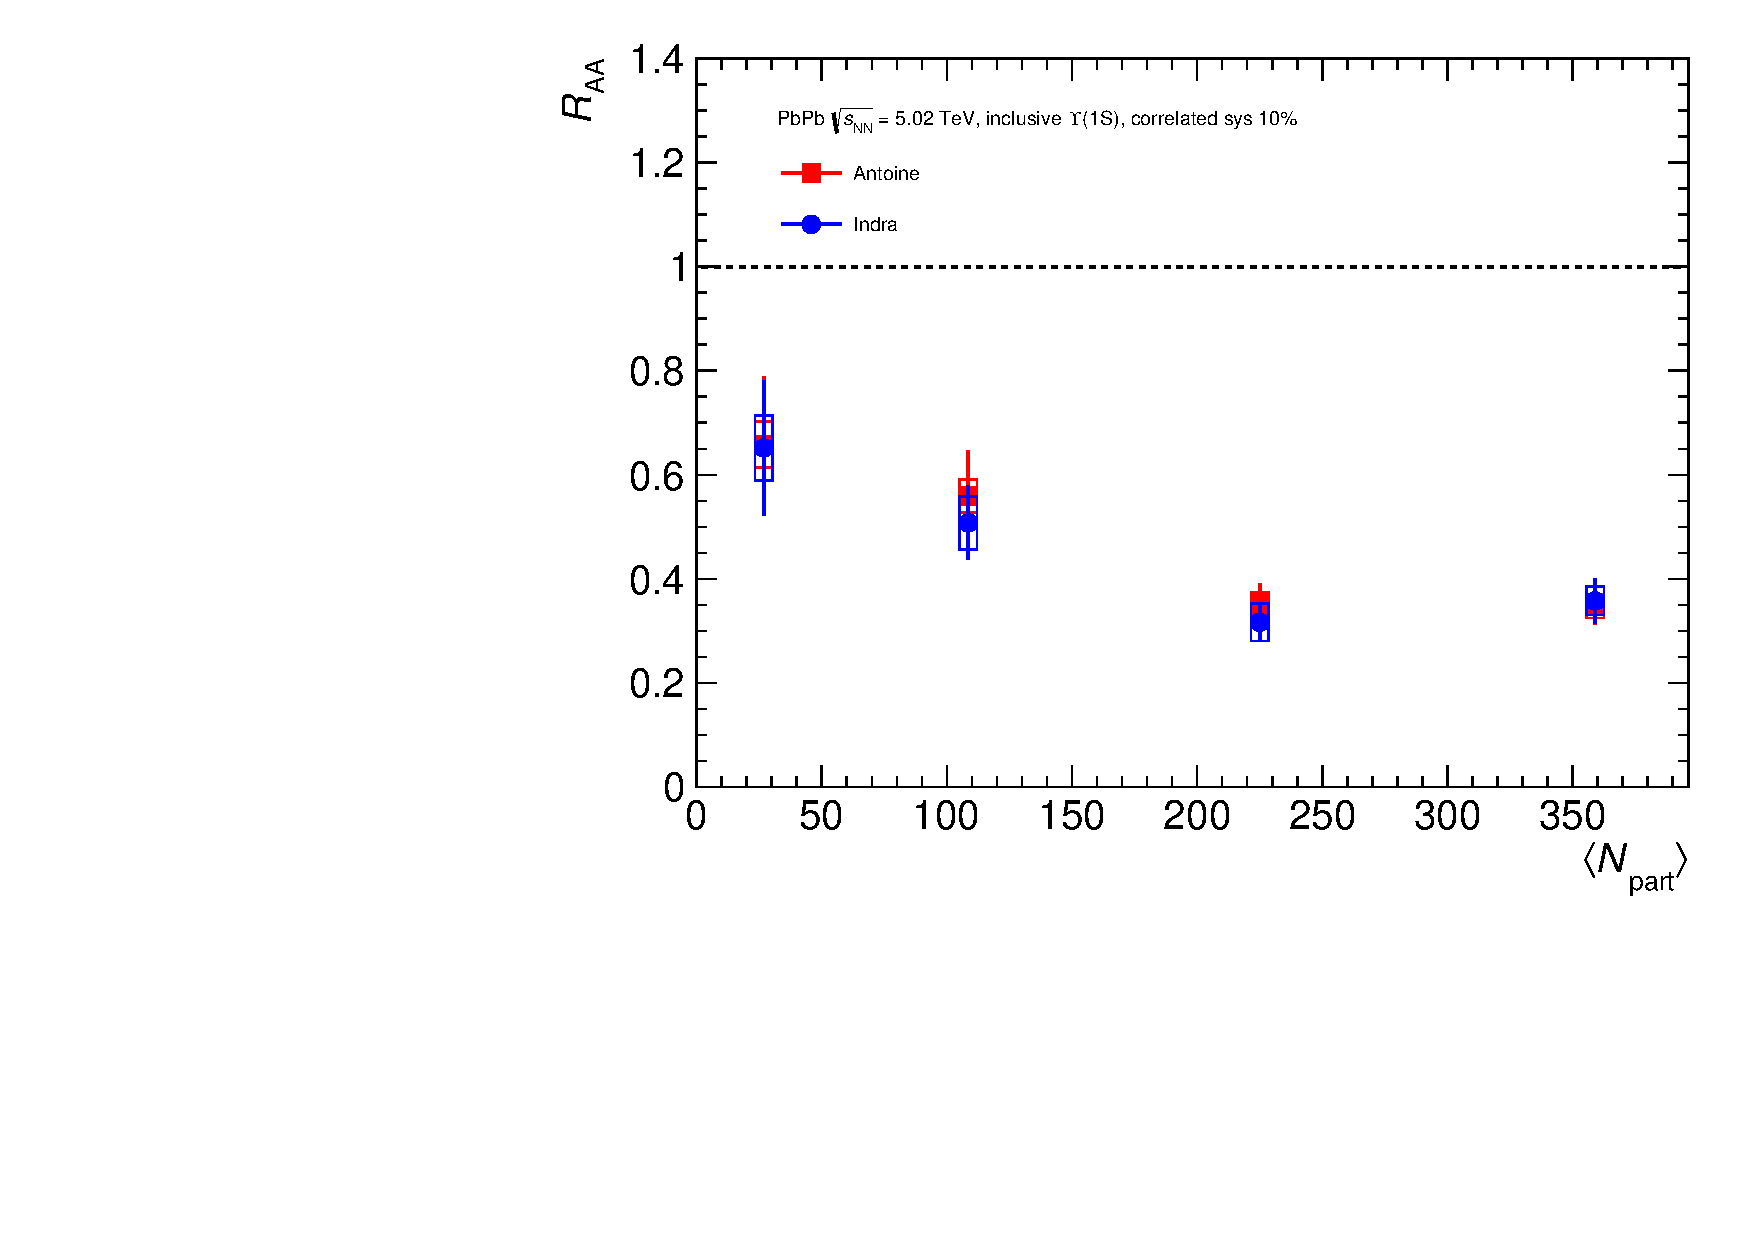
\includegraphics[width=6cm]{Results/Indra_results_2016_06_08/RAA_cent.pdf}
%  \centering 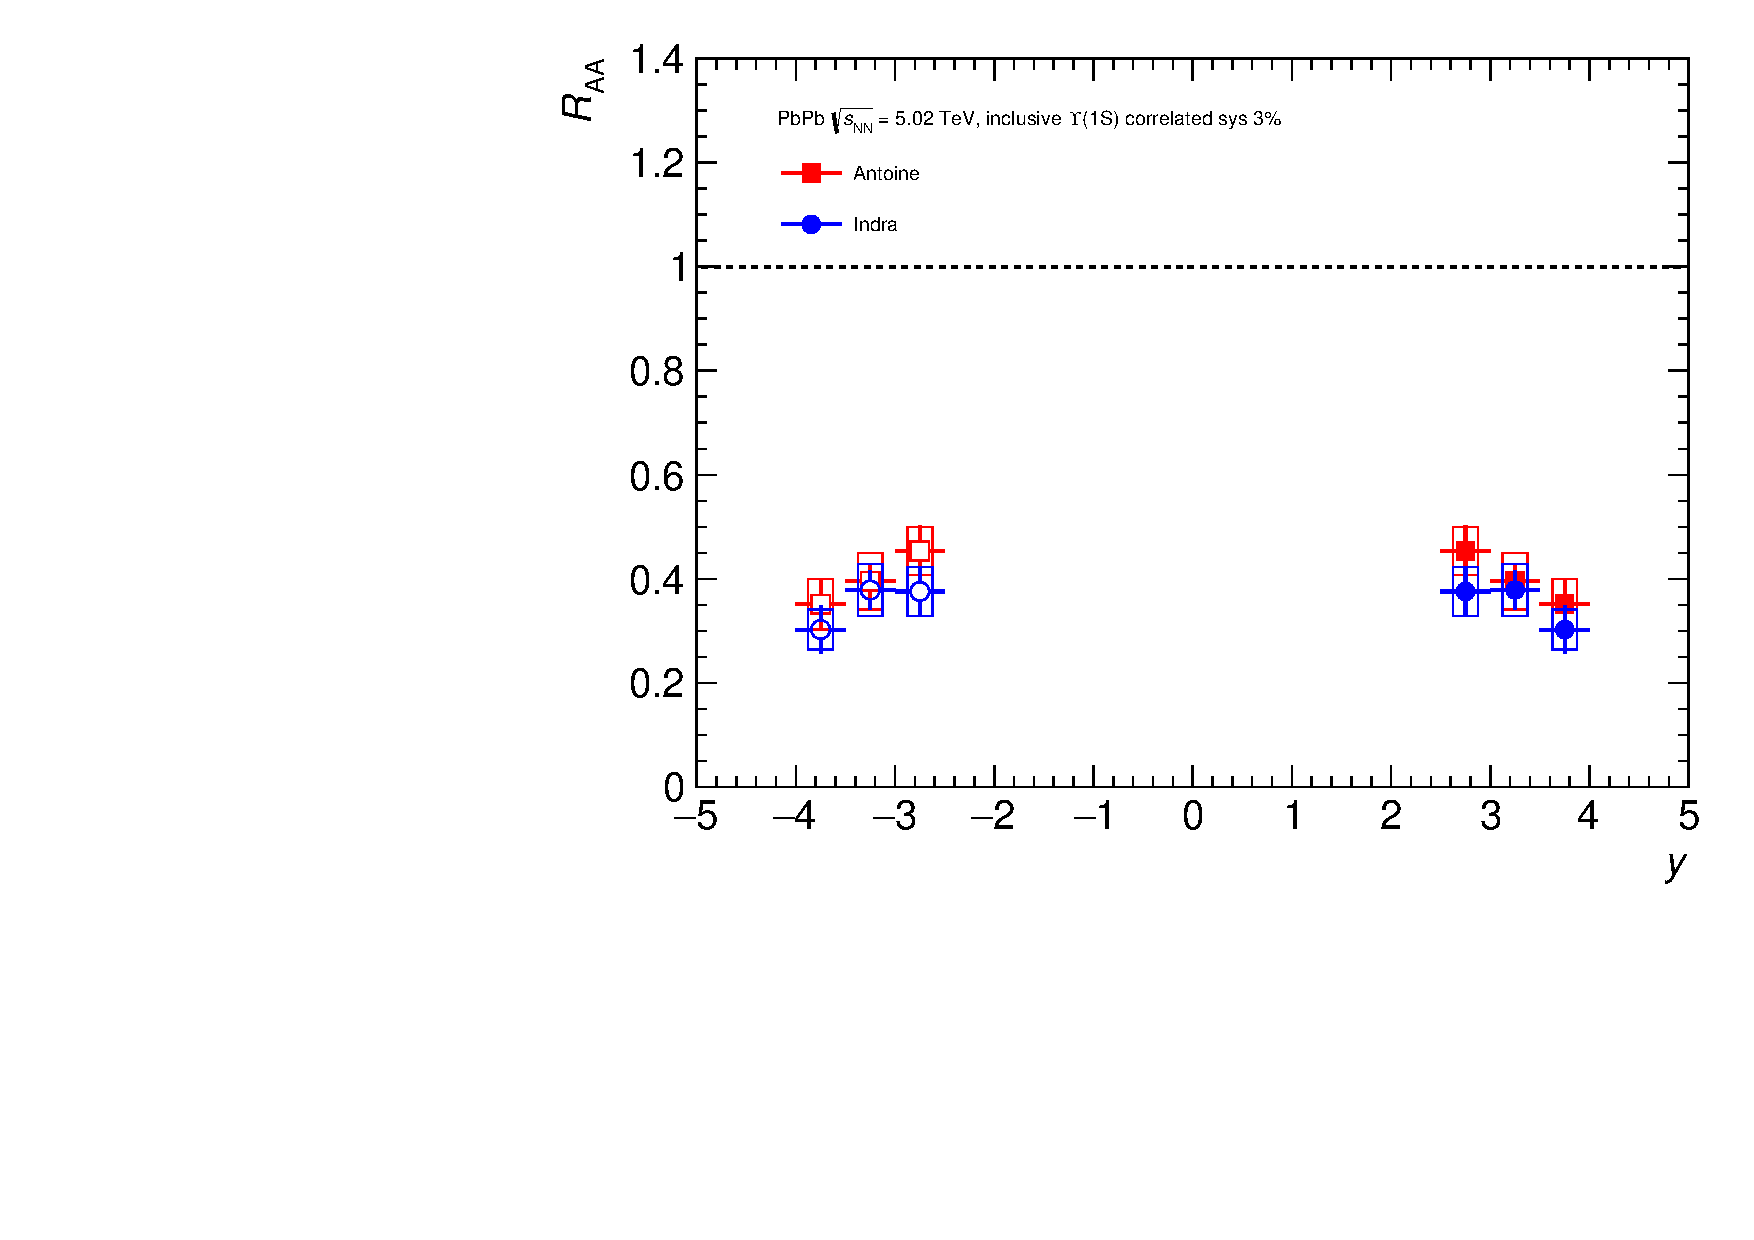
\includegraphics[width=6cm]{Results/Indra_results_2016_06_08/RAA_rap.pdf}
%  \caption{\scriptsize $R_{\rm AA}$ vs $\langle N_{\rm part} \rangle$}
%\end{figure}       


\begin{figure}[!h]
  \centering 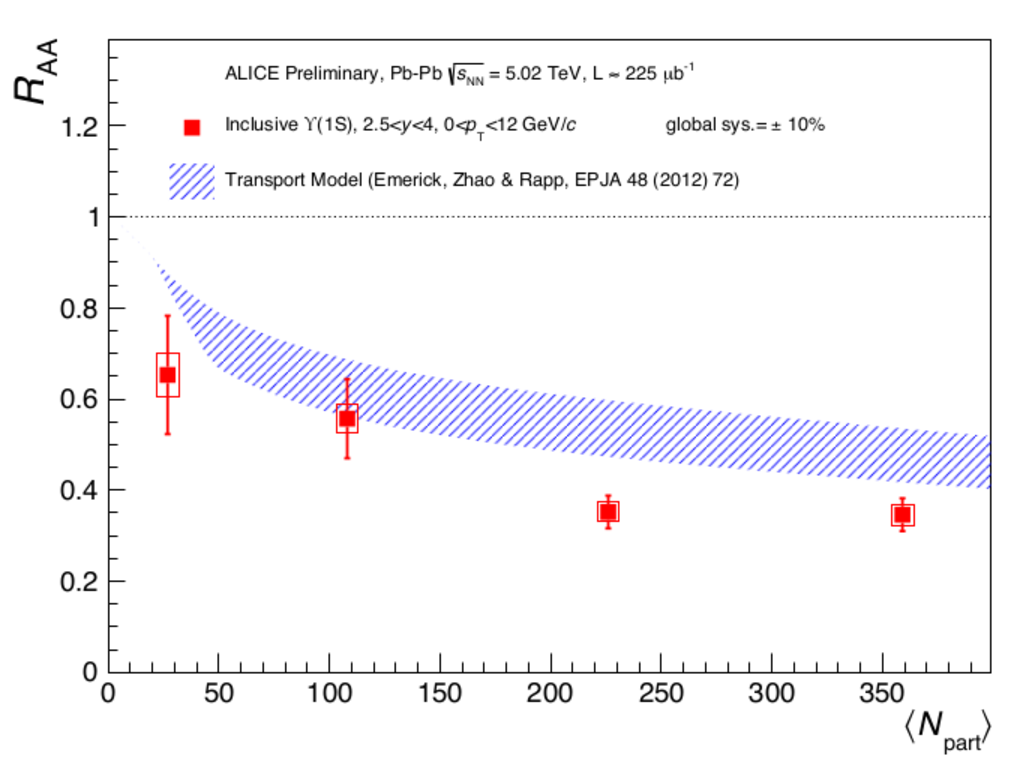
\includegraphics[width=6.5cm]{Results/Antoine_results_2016_06_07/RAA_vs_cent_5TeV_model_Emerick.pdf}
  \caption{\label{rapp}\scriptsize $R_{\rm AA}$ vs centrality, Rapp \& al model}
\end{figure} 
      

\begin{figure}[!h]
  \centering 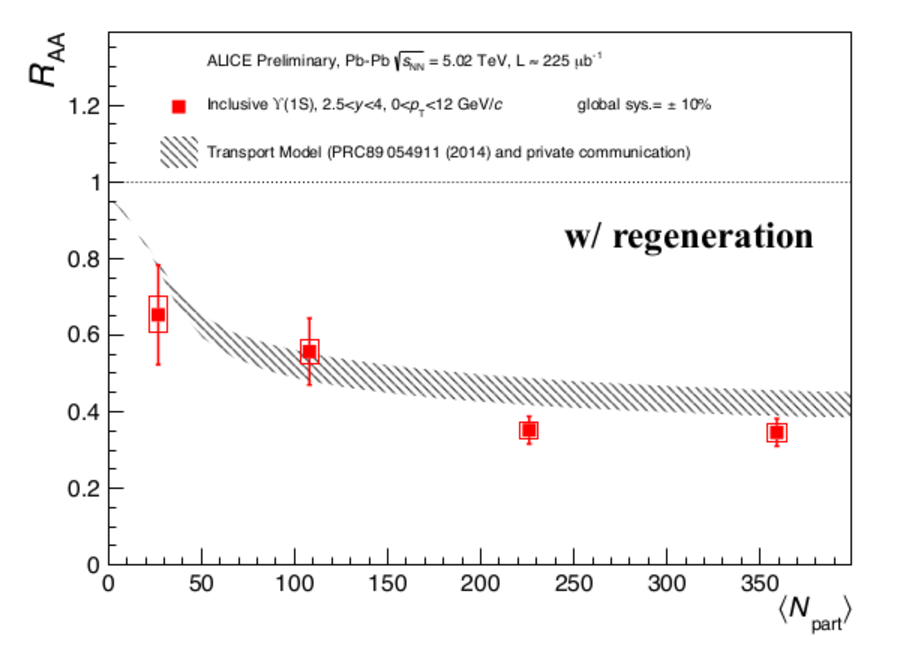
\includegraphics[width=6.5cm]{Results/Antoine_results_2016_06_07/RAA_vs_cent_5TeV_model_Zhou_wt_regeration.pdf}
  \centering 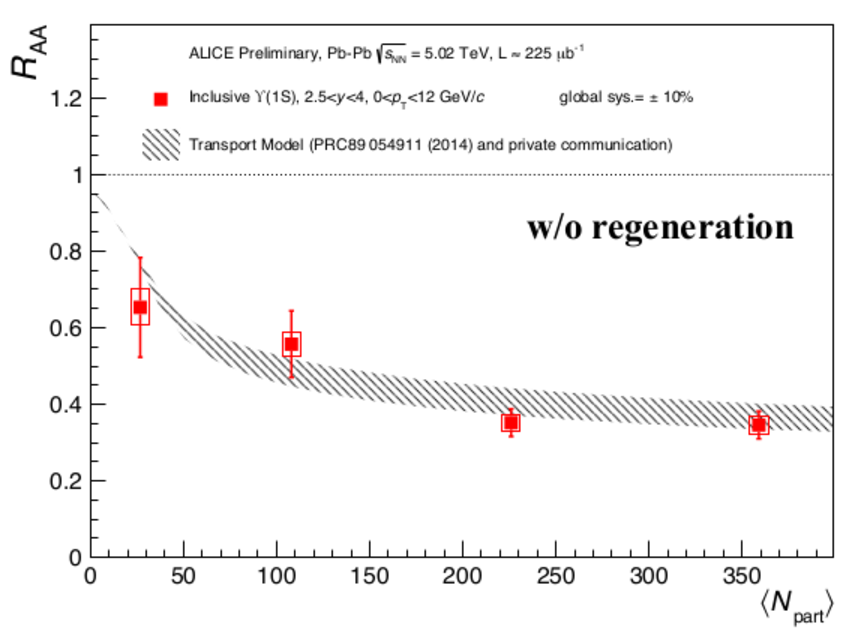
\includegraphics[width=6.5cm]{Results/Antoine_results_2016_06_07/RAA_vs_cent_5TeV_model_Zhou_wo_regeration.pdf}
  \caption{\label{kai}\scriptsize $R_{\rm AA}$ vs centrality, Kai \& al model}
\end{figure}       


\begin{table}[htb]
\begin{center}
  {\scriptsize
    \begin{tabular} { c | c | c }
      \hline
      centrality   & $R_{\rm AA}$ (Antoine) &  $R_{\rm AA}$ (Indra) \\\hline
      $[0-10]\%$   & $0.35 \pm 0.04 (10.43\%) \pm 0.02 (6.52\%) \pm 0.03 (9.60\%)$ & $0.36 \pm 0.04 (12.01\%) \pm 0.03 (7.63\%) \pm 0.03 (9.60\%)$ \\
      $[10-30]\%$  & $0.35 \pm 0.04 (10.32\%) \pm 0.02 (6.05\%) \pm 0.03 (9.60\%)$ &$0.32 \pm 0.04 (11.38\%) \pm 0.04 (11.29\%) \pm 0.03 (9.60\%)$ \\
      $[30-50]\%$  & $0.56 \pm 0.09 (15.60\%) \pm 0.03 (5.74\%) \pm 0.05 (9.60\%)$ &$0.51 \pm 0.07 (14.00\%) \pm 0.05 (10.11\%) \pm 0.05 (9.60\%)$ \\
      $[50-90]\%$  & $0.65 \pm 0.13 (20.00\%) \pm 0.05 (6.66\%) \pm 0.06 (9.60\%)$ &$0.65 \pm 0.13 (20.00\%) \pm 0.06 (9.61\%) \pm 0.06 (9.60\%)$ \\\hline
    \end{tabular}
  }
    \caption{\label{raavaluescent} Centrality dependence of \ups $R_{\rm AA}$ at 5.02 TeV}
\end{center}
\end{table}


\begin{table}[htb]
\begin{center}
  {\scriptsize
    \begin{tabular} { c | c | c }
      \hline
      rapidity     & $R_{\rm AA}$  (Antoine) & $R_{\rm AA}$  (Indra)\\\hline
      $[2.5-3.0]$  & $0.45 \pm 0.05 (10.80\%) \pm 0.05 (10.14\%) \pm 0.01 (3.25\%)$ & $0.38 \pm 0.05 (12.43\%) \pm 0.05 (12.58\%) \pm 0.01 (3.25\%)$ \\
      $[3.0-3.5]$  & $0.40 \pm 0.03 (8.76\%) \pm 0.05 (13.72\%) \pm 0.01 (3.25\%)$ &$0.38 \pm 0.04 (10.00\%) \pm 0.05 (13.15\%) \pm 0.01 (3.25\%)$ \\
      $[3.5-4.0]$  & $0.45 \pm 0.05 (10.80\%) \pm 0.05 (10.14\%) \pm 0.01 (3.25\%)$ &$0.30 \pm 0.05 (15.13\%) \pm 0.04 (12.69\%) \pm 0.01 (3.25\%)$ \\\hline
    \end{tabular}
  }
    \caption{\label{raavaluesy} Rapidity dependence of \ups $R_{\rm AA}$ at 5.02 TeV}
\end{center}
\end{table}
